\documentclass[class=article, crop=true]{standalone}
\usepackage{tikz}
\usepackage{subcaption}
\usepackage[subpreambles=true]{standalone}
\begin{document}

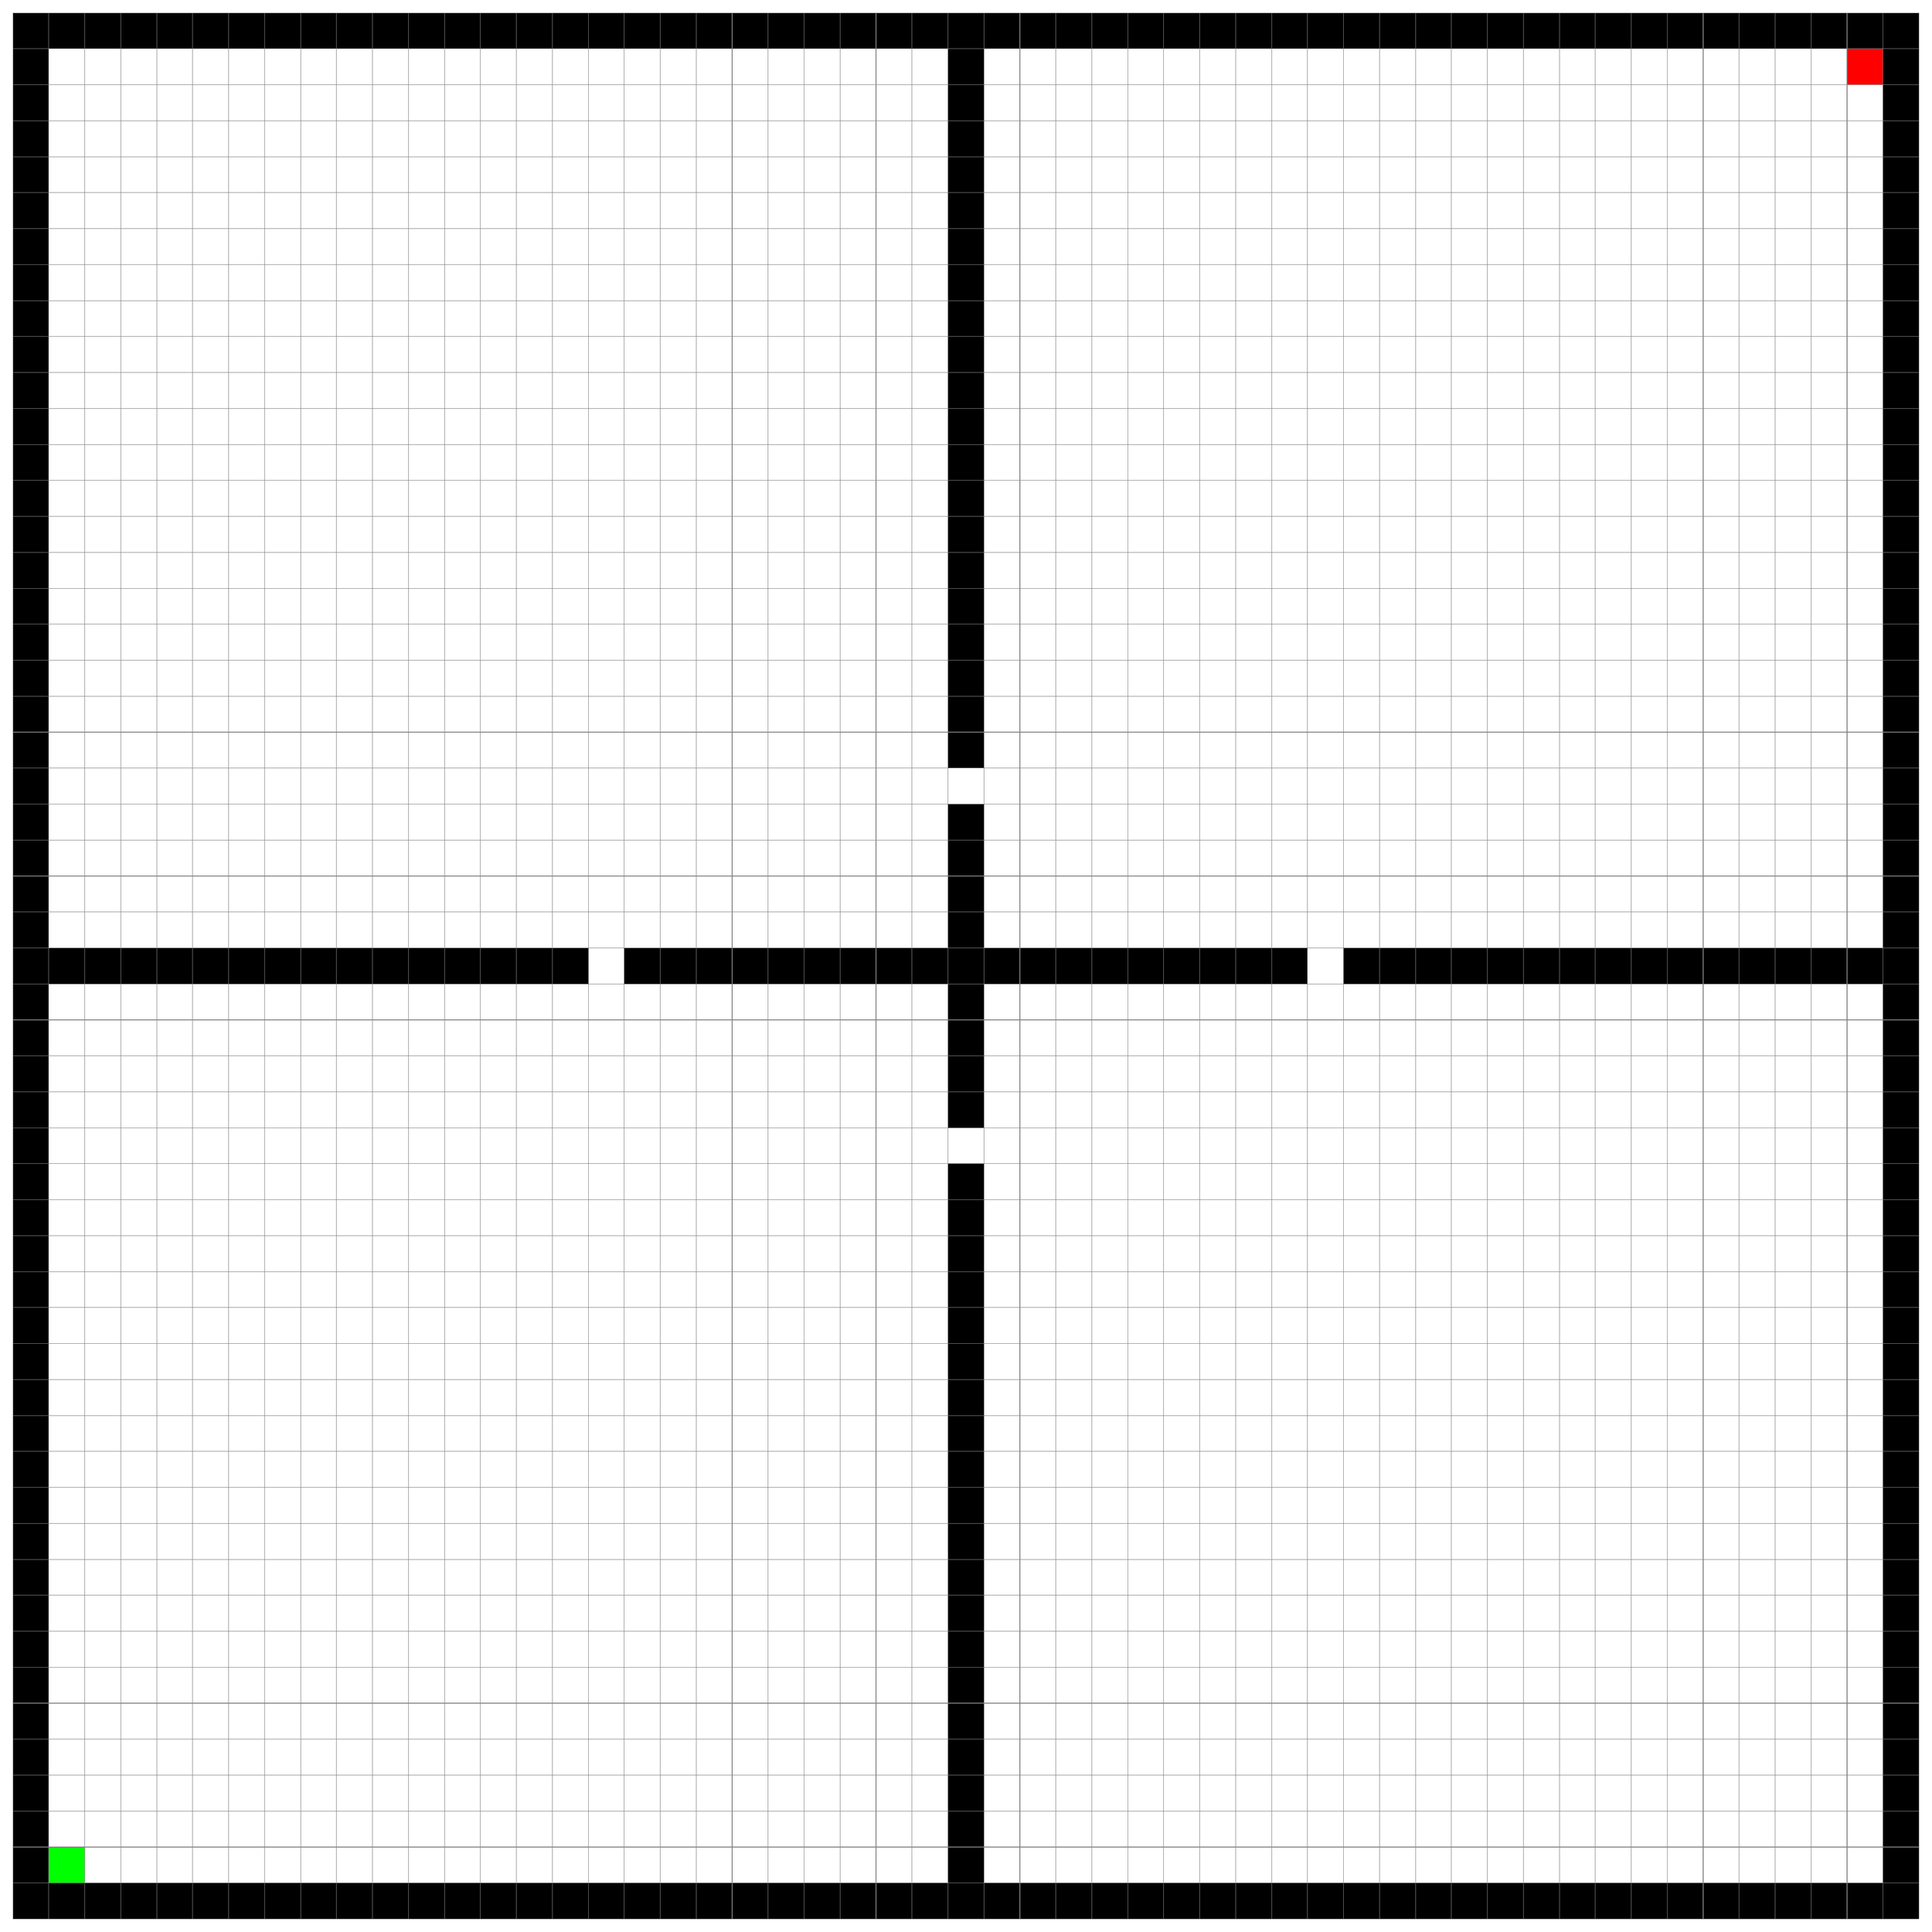
\begin{tikzpicture}
% Background
\fill[white] (-26.5, -26.5) rectangle (26.5, 26.5);

% Outer Lines
\fill[black] (-26.5, -26.5) -- (26.5, -26.5) -- (26.5, -25.5) -- (-26.5, -25.5) -- cycle;
\fill[black] (25.5, -26.5) -- (26.5, -26.5) -- (26.5, 26.5) -- (25.5, 26.5) -- cycle;
\fill[black] (-26.5, 26.5) -- (26.5, 26.5) -- (26.5, 25.5) -- (-26.5, 25.5) -- cycle;
\fill[black] (-25.5, -26.5) -- (-26.5, -26.5) -- (-26.5, 26.5) -- (-25.5, 26.5) -- cycle;

% Inner Lines
\fill[black] (-26.5, 0.5) -- (-10.5, 0.5) -- (-10.5, -0.5) -- (-26.5, -0.5) -- cycle;
\fill[black] (-9.5, 0.5) -- (9.5, 0.5) -- (9.5, -0.5) -- (-9.5, -0.5) -- cycle;
\fill[black] (10.5, 0.5) -- (26.5, 0.5) -- (26.5, -0.5) -- (10.5, -0.5) -- cycle;

\fill[black] (-0.5, -26.5) -- (0.5, -26.5) -- (0.5, -5.5) -- (-0.5, -5.5) -- cycle;
\fill[black] (-0.5, -4.5) -- (0.5, -4.5) -- (0.5, 4.5) -- (-0.5, 4.5) -- cycle;
\fill[black] (-0.5, 26.5) -- (0.5, 26.5) -- (0.5, 5.5) -- (-0.5, 5.5) -- cycle;

% Starting Point
\fill[red] (24.5, 24.5) -- (25.5, 24.5) -- (25.5, 25.5) -- (24.5, 25.5) -- cycle;
% Goal Point
\fill[green] (-24.5, -24.5) -- (-25.5, -24.5) -- (-25.5, -25.5) -- (-24.5, -25.5) -- cycle;

% Grid
\foreach \x in {-26.5, ..., 26.5} {\draw[gray, thin] (\x, -26.5) -- (\x, 26.5);}
\foreach \y in {-26.5, ..., 26.5} {\draw[gray, thin] (-26.5, \y) -- (26.5, \y);}
\end{tikzpicture}

\end{document}